\section{Câu 5}
     Thực hiện calib camera bằng phương pháp trực tiếp sau đó tìm lại ma trận thông số nội và ngoại, so sánh với phương pháp gián tiếp đã làm ở câu 3.
     \subsection{Cơ sở lý thuyết}
          \hspace*{0.6cm}Quá trình hiệu chỉnh camera bằng phương pháp trực tiếp là đi tìm các thông số trong ma trận chiếu (projection matrix), khi ta đã
          biết tọa độ các điểm $A_1, A_2, \dots, A_n$ trong hệ tọa độ vật và tọa độ tương ứng $a_1, a_2, \dots, a_n$ của chúng trên mặt phẳng ảnh.\\ % tài liệu tham khảo sách thầy Hạnh
          \hspace*{0.6cm}Giả sử bỏ qua các điểm distortion, có 12 thông số cần tìm trong ma trận hình chiếu. Giả sử các điểm trong tọa độ thực là $A_i = [X_i \quad Y_i \quad Z_i \quad 1]^T$ biết trước có ảnh $a_i = [u_i \quad v_i]$ biết trước ($i = 1, 2, 3, \dots$). Ta có công thức chuyển đổi
          % Phần đầu: ma trận biến đổi affine 3D
          \begin{align}
               \begin{bmatrix}
               su \\
               sv \\
               s
               \end{bmatrix}
               &=
               \begin{bmatrix}
               m_{11} & m_{12} & m_{13} & m_{14} \\
               m_{21} & m_{22} & m_{23} & m_{24} \\
               m_{31} & m_{32} & m_{33} & m_{34}
               \end{bmatrix}
               \begin{bmatrix}
               X \\ Y \\ Z \\ 1
               \end{bmatrix}
               \Rightarrow \quad
               \begin{cases}
               su = m_{11}X + m_{12}Y + m_{13}Z + m_{14} \\
               sv = m_{21}X + m_{22}Y + m_{23}Z + m_{24} \\
               s  = m_{31}X + m_{32}Y + m_{33}Z + m_{34}
               \end{cases}
               \label{c5_eq1}
          \end{align}
          \hspace*{0.6cm}Từ (\ref{c5_eq1}) rút ra biểu thức cho $u$ và $v$
          \begin{align*}
               u &= \dfrac{m_{11}X + m_{12}Y + m_{13}Z + m_{14}}{m_{31}X + m_{32}Y + m_{33}Z + m_{34}} \\
               v &= \dfrac{m_{21}X + m_{22}Y + m_{23}Z + m_{24}}{m_{31}X + m_{32}Y + m_{33}Z + m_{34}}
          \end{align*}
          Khai triển và biến đổi chuyển vế ta có biểu thức
          \begin{align}
               0 &= m_{11}X + m_{12}Y + m_{13}Z + m_{14} - m_{31}uX - m_{32}uY - m_{33}uZ - m_{34}u \\
               0 &= m_{21}X + m_{22}Y + m_{23}Z + m_{24} - m_{31}vX - m_{32}vY - m_{33}vZ - m_{34}v
          \end{align}
          Đưa về dạng ma trận $\mathbf{Ax} = \mathbf{0}$  ta có
          \begin{equation}
               \left[
               \begin{array}{cccccccccccc}
                    X_1 & Y_1 & Z_1 & 1 & 0   & 0   & 0   & 0 & -u_1X_1 & -u_1Y_1 & -u_1Z_1 & -u_1 \\
                    0   & 0   & 0   & 0 & X_1 & Y_1 & Z_1 & 1 & -v_1X_1 & -v_1Y_1 & -v_1Z_1 & -v_1 \\
                    \vdots & \vdots & \vdots & \vdots & \vdots & \vdots & \vdots & \vdots & \vdots & \vdots & \vdots & \vdots \\
                    X_n & Y_n & Z_n & 1 & 0   & 0   & 0   & 0 & -u_nX_n & -u_nY_n & -u_nZ_n & -u_n \\
                    0   & 0   & 0   & 0 & X_n & Y_n & Z_n & 1 & -v_nX_n & -v_nY_n & -v_nZ_n & -v_n
               \end{array}
               \right]
               \begin{bmatrix}
                    m_{11} \\
                    m_{12} \\
                    m_{13} \\
                    m_{14} \\
                    m_{21} \\
                    m_{22} \\
                    m_{23} \\
                    m_{24} \\
                    m_{31} \\
                    m_{32} \\
                    m_{33} \\
                    m_{34}
               \end{bmatrix}
               =
               \begin{bmatrix}
                    0 \\
                    0 \\
                    \vdots \\
                    0 \\
                    0
               \end{bmatrix}
          \end{equation}
          \hspace*{0.6cm}Giải hệ này tìm ra các hệ số của ma trận hình chiếu sử dụng phương pháp SVD (Singular Value Decomposition). Rồi từ đó phân tách ra thành ma trận thông số nội $K$, ma trận xoay $R$ và vector tịnh tiến $T$.
     \subsection{Các bước thực hiện}
          Quá trình thực hiện bao gồm các bước sau:
          \begin{itemize}
               \item Bước 1: Sử dụng một mặt phẳng chứa một hệ tọa độ xác định như hình, chiều dài mỗi ô trên hệ tọa độ là 5mm.
               \begin{figure}[h]
               \centering
               \begin{minipage}{0.48\textwidth}
                    \centering
                    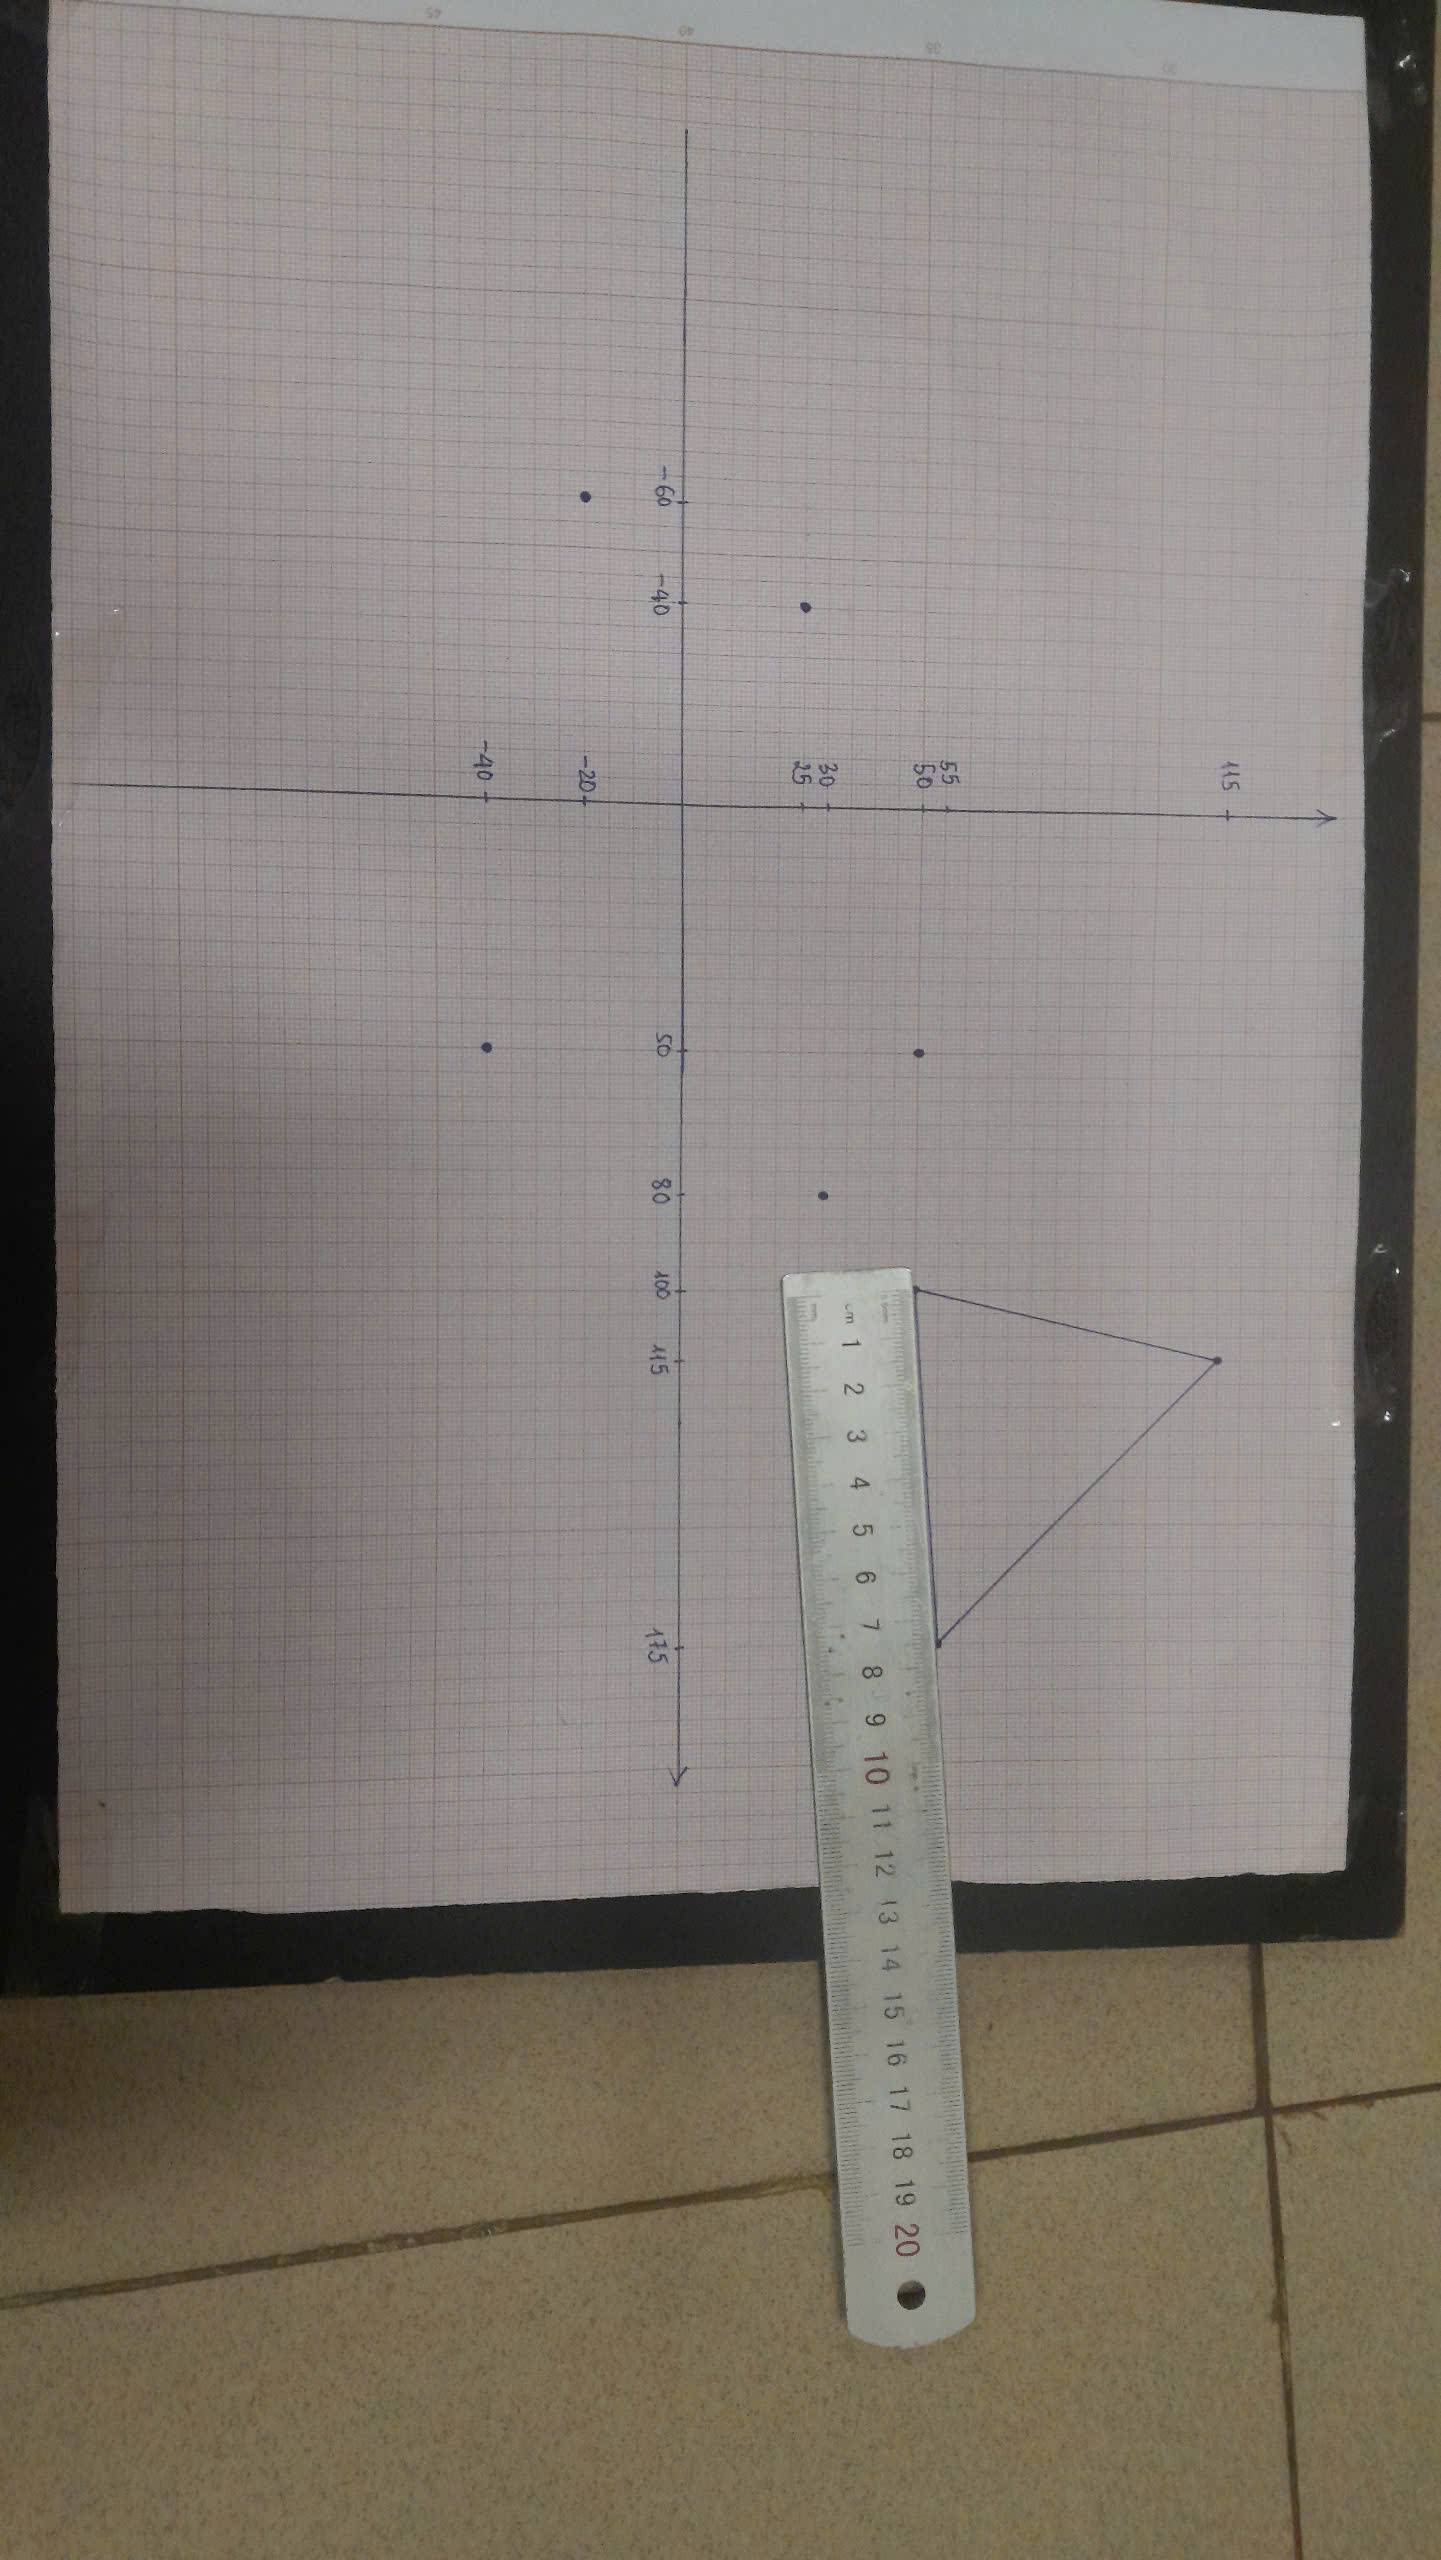
\includegraphics[width=0.7\textwidth]{pictures/chapter5/c5_p01_setup1.jpg}
               \end{minipage}
               \hfill
               \begin{minipage}{0.48\textwidth}
                    \centering
                    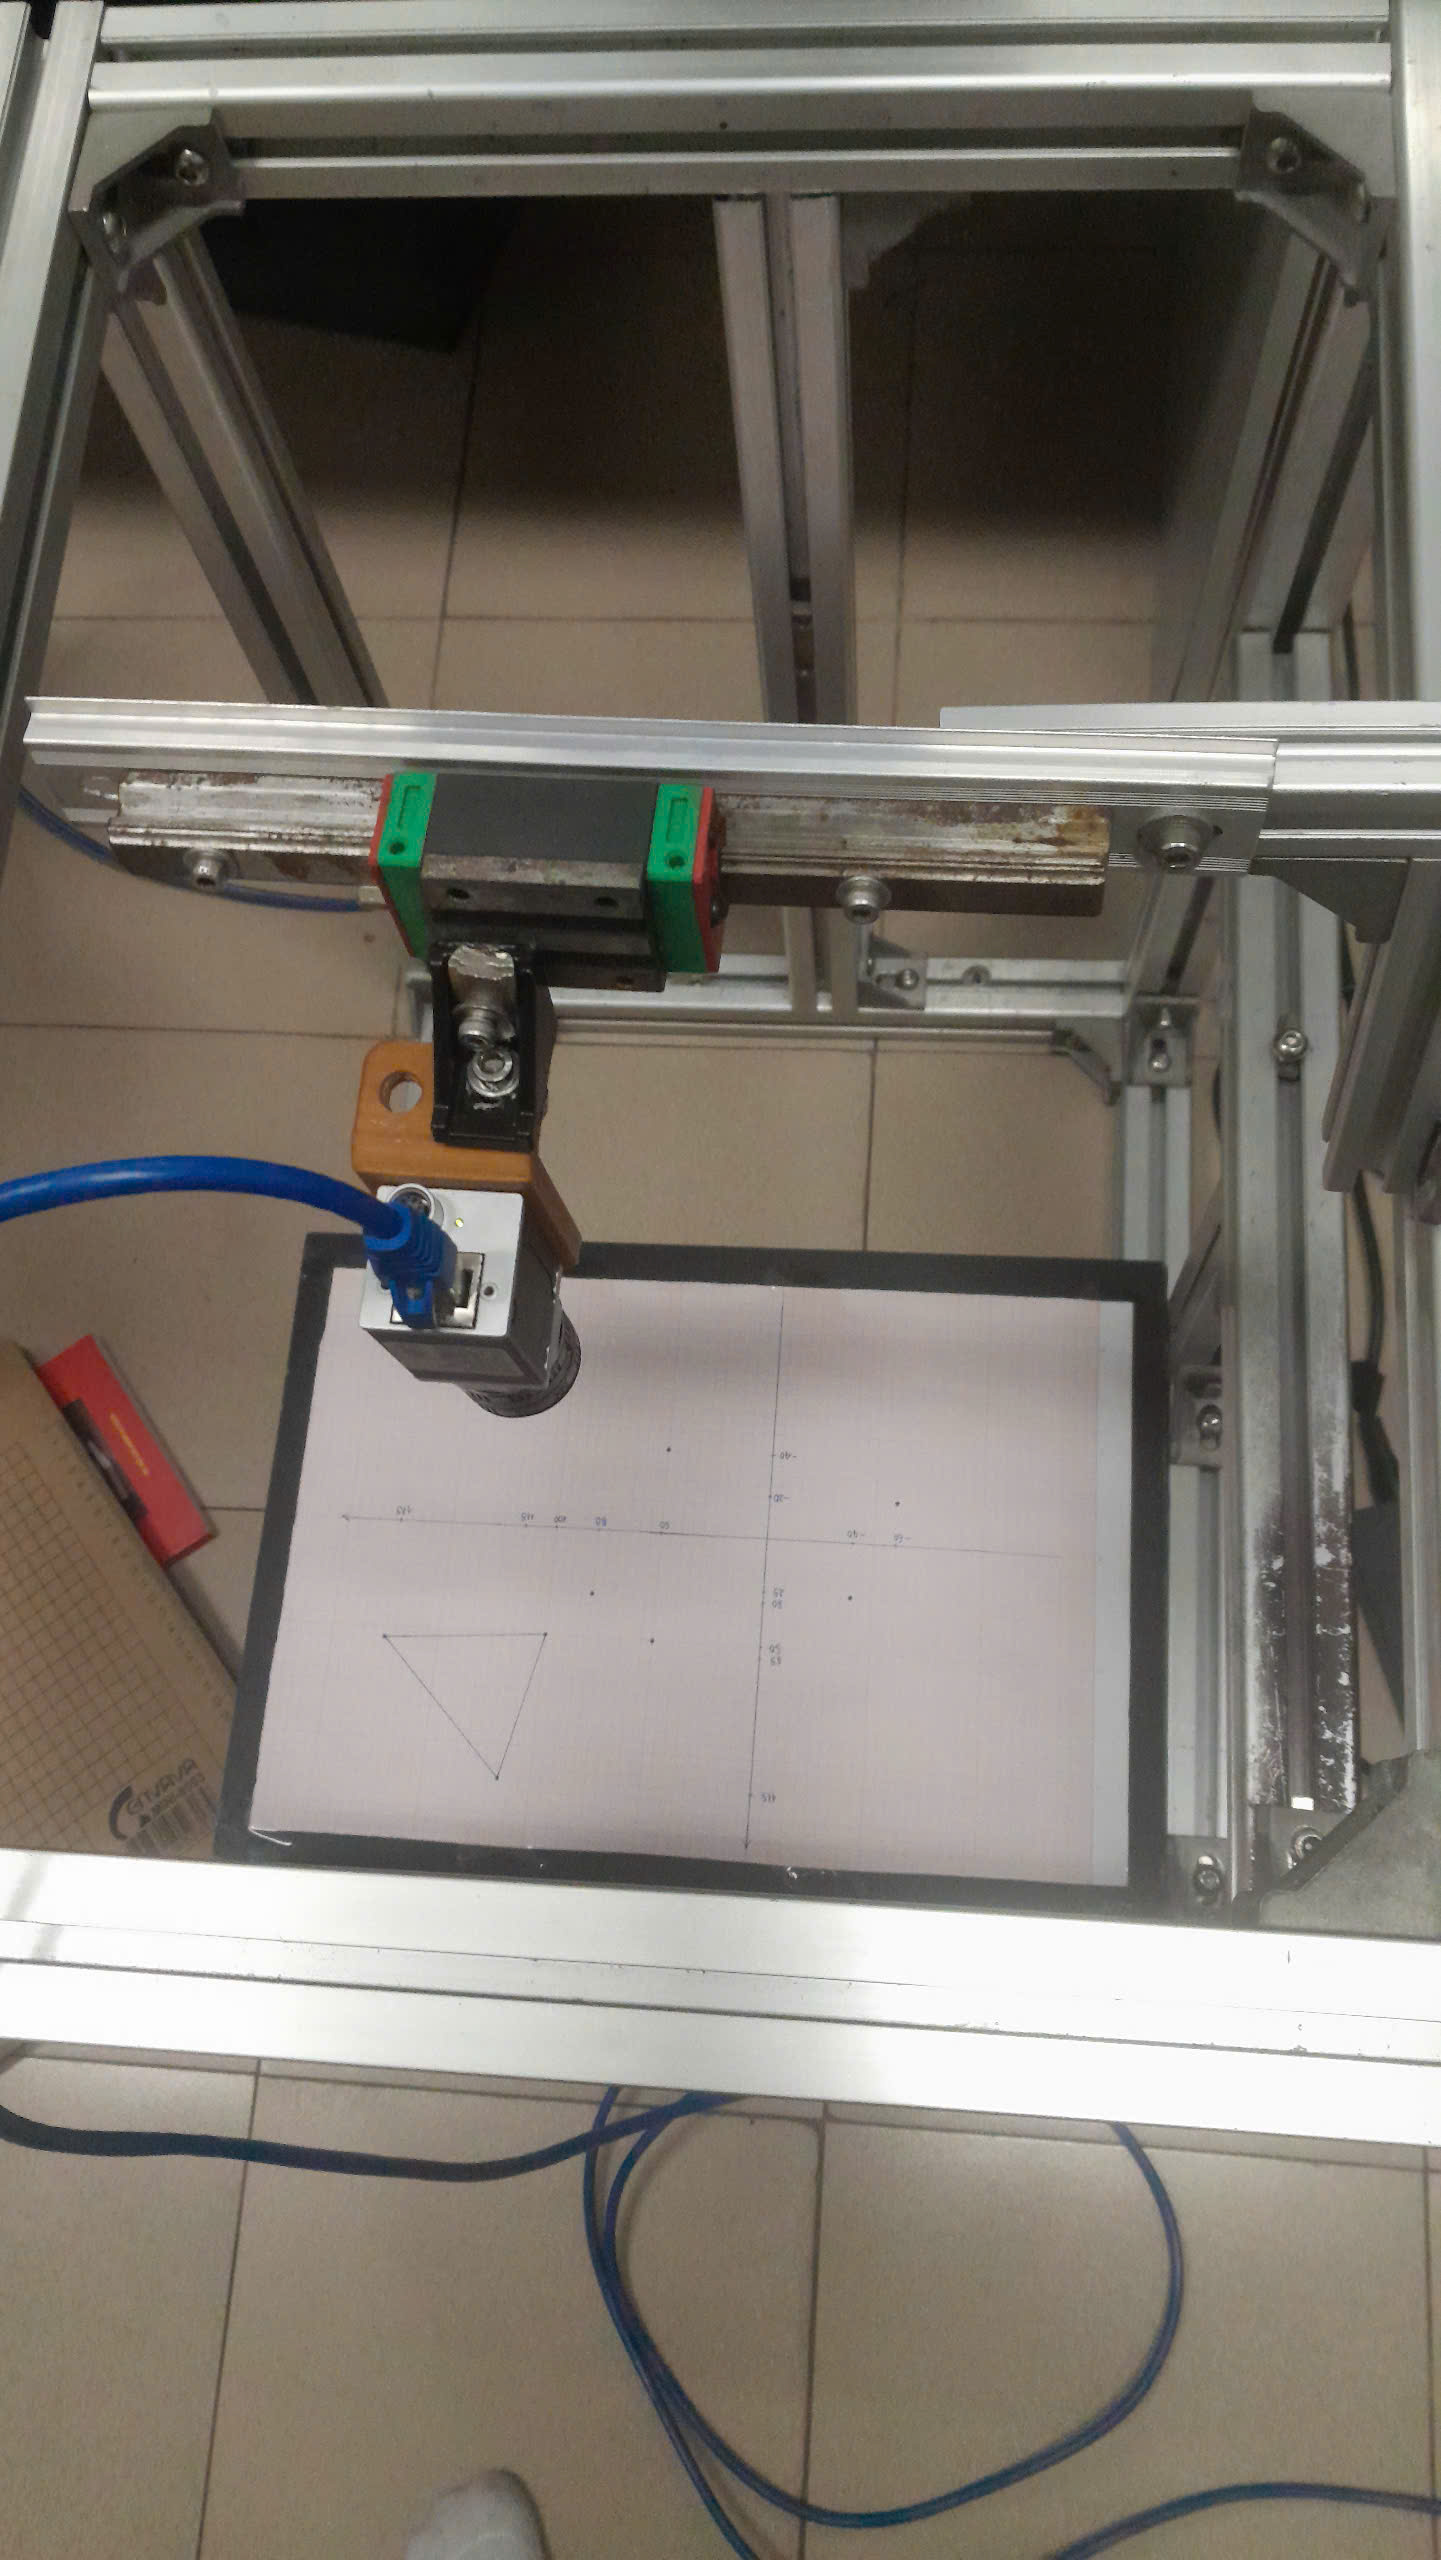
\includegraphics[width=0.7\textwidth]{pictures/chapter5/c5_p01_setup2.jpg}
               \end{minipage}
               \caption{Mặt phẳng hệ tọa độ dùng để calib camera trực tiếp}
               \label{c5_pic01_setup}
               \end{figure}
               \item Bước 2: Chấm các điểm có tọa độ xác định trên mặt phẳng hệ tọa độ, ghi lại các tọa độ thực tế $X_i, Y_i$ của các điểm này trong hệ tọa độ không gian.
               \item Bước 3: Dùng thước dây đo khoảng cách từ camera đến mặt phẳng hệ tọa độ để lấy giá trị $Z_i$ cho các điểm đã chấm. Với mỗi độ cao, các điểm đã chấm trên mặt phẳng sẽ có tọa độ trong không gian là $A_i = [X_i \quad Y_i \quad Z_i \quad 1]^T$.
               \begin{figure}[H]
                    \centering
                    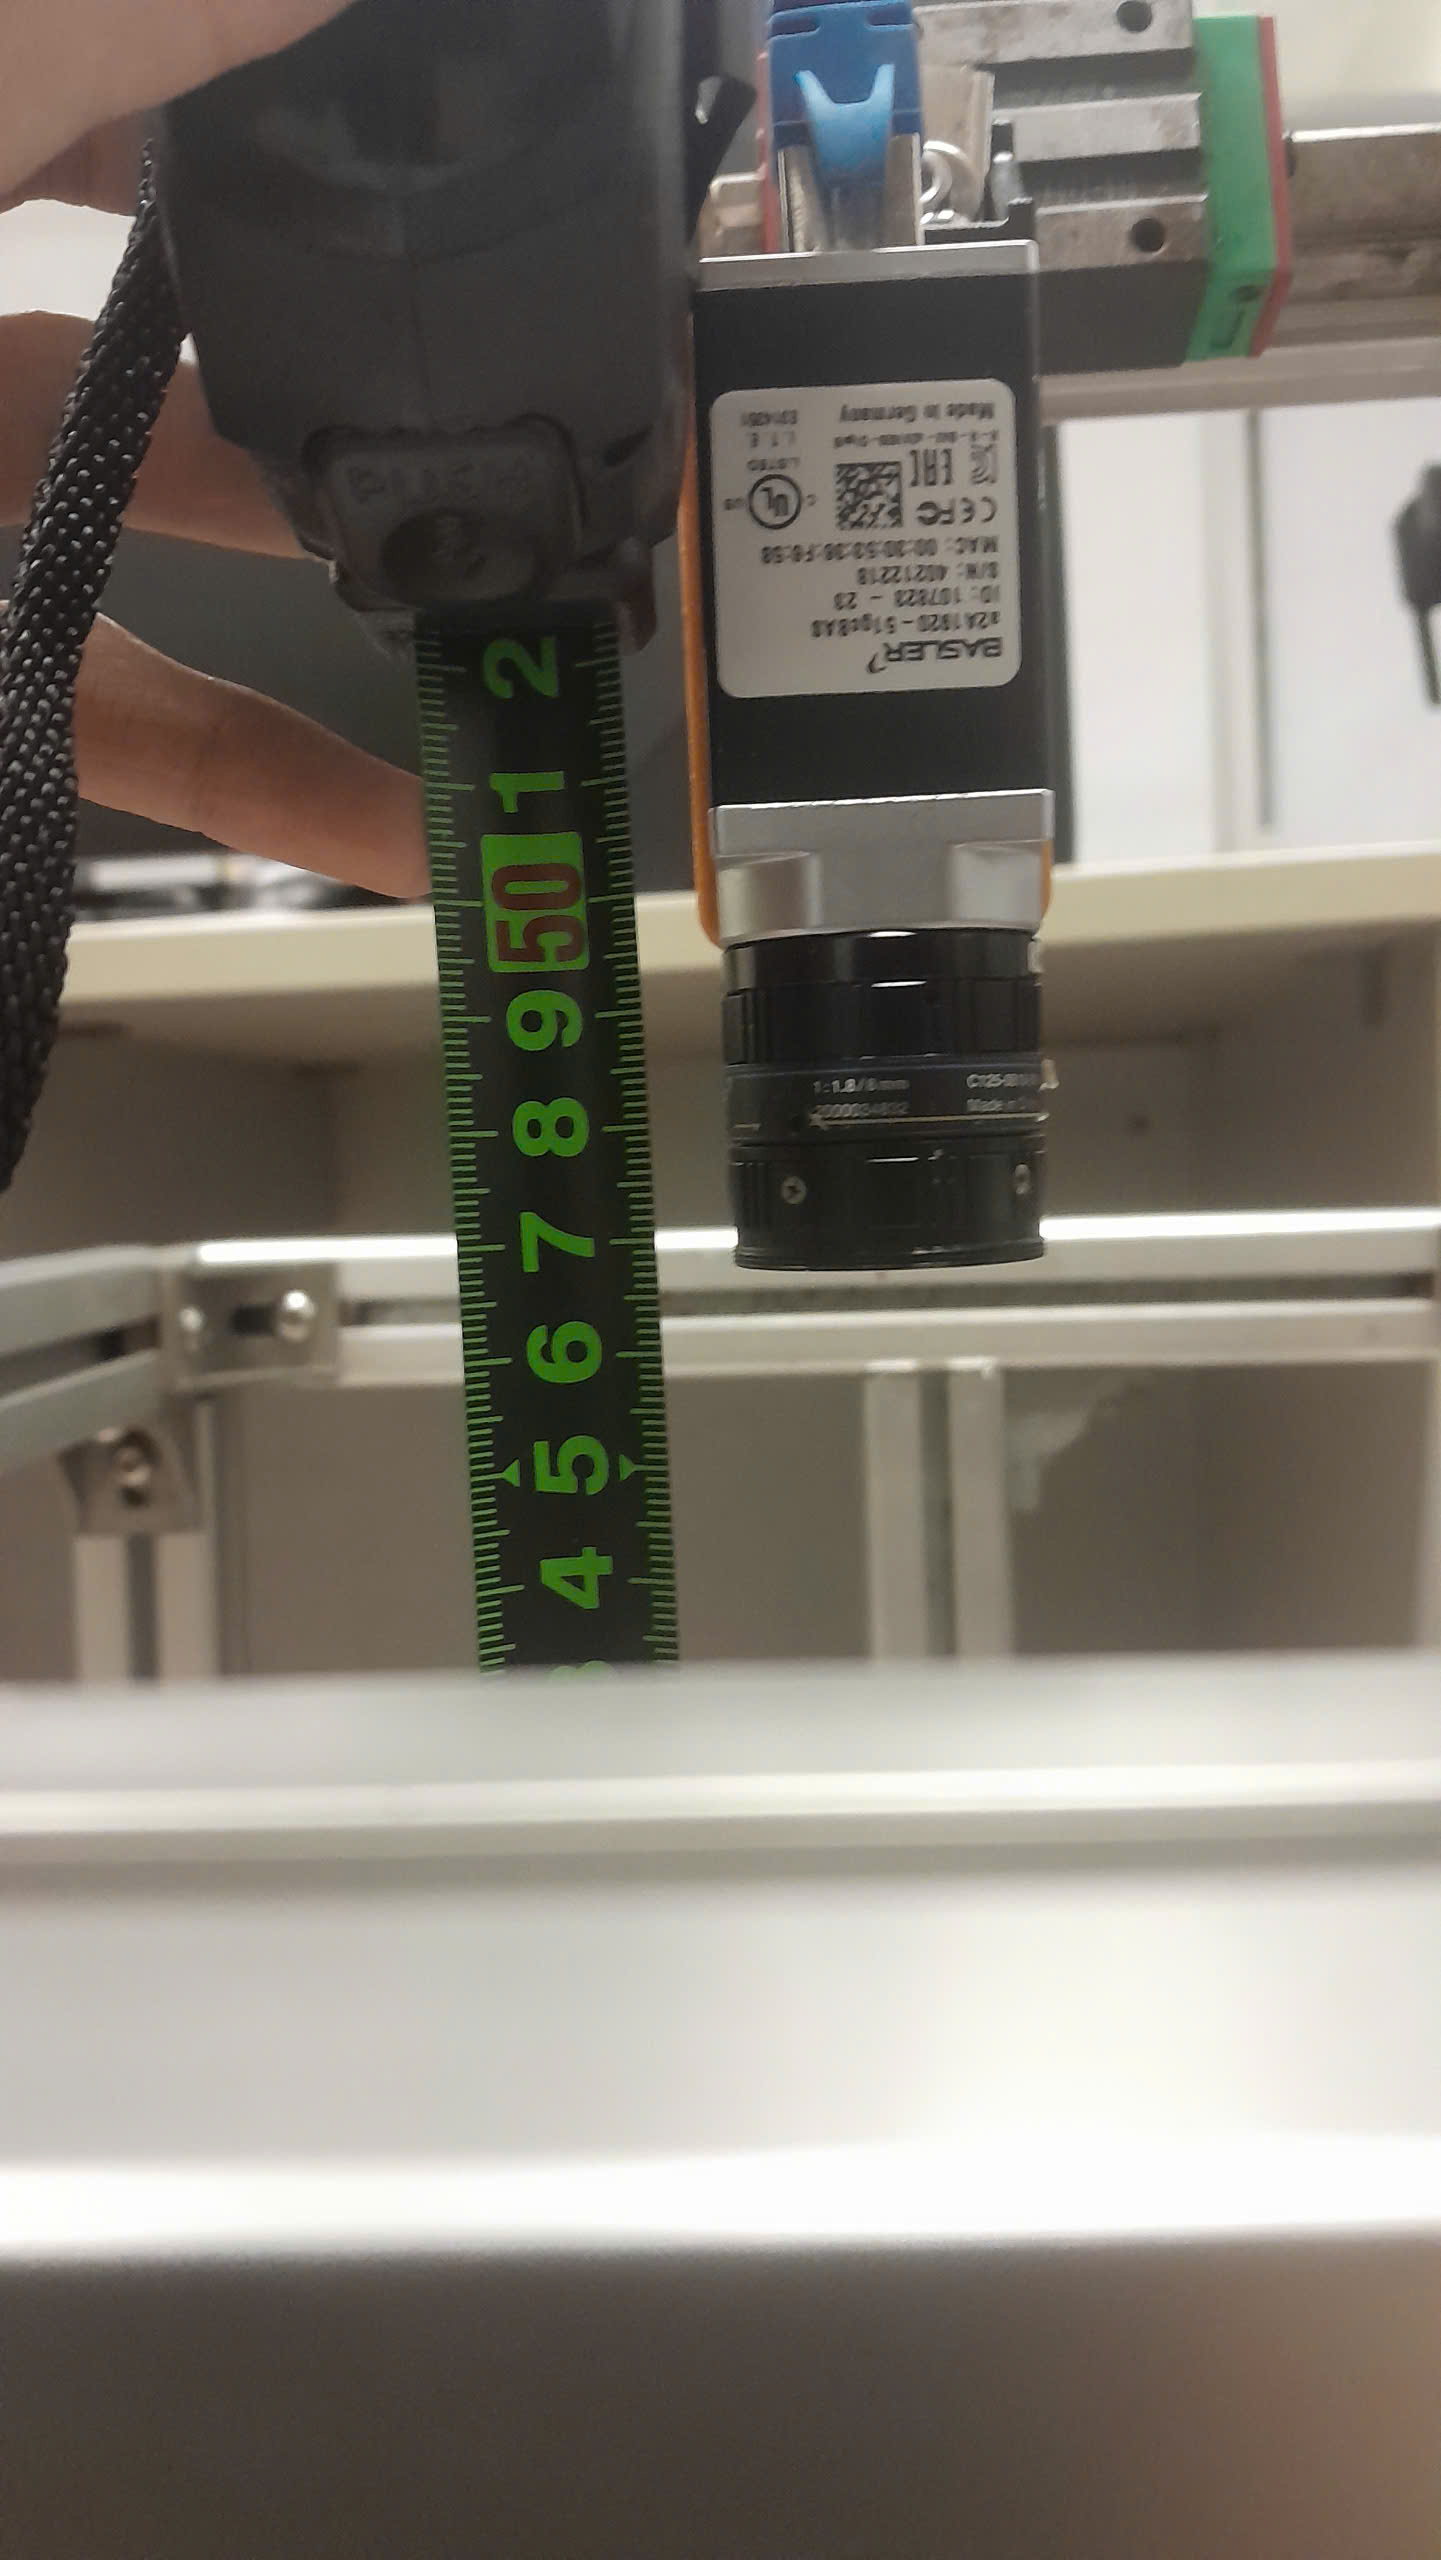
\includegraphics[width=0.5\textwidth]{pictures/chapter5/c5_p01_h467.jpg}
                    \caption{Dùng thước dây đo độ cao từ camera đến mặt phẳng hệ tọa độ}
                    \label{c5_pic02_height}
               \end{figure}
               \item Bước 4: Chụp ảnh các điểm đã chấm từ camera, sử dụng code để lấy tọa độ ảnh $u_i, v_i$ tương ứng của các điểm này trên mặt phẳng ảnh.
          \end{itemize}


